\documentclass{beamer}
\usetheme{default}
\usecolortheme{default}

%% custom color theme. 
\definecolor{sidebartop}{RGB}{133,135,86}
\definecolor{sidebar}{RGB}{177,179,115}
\definecolor{sidebarbot}{RGB}{211,213,136}
\definecolor{title}{RGB}{241,243,186}
\setbeamertemplate{sidebar canvas left}[vertical shading][top=sidebar,bottom=sidebarbot]
\setbeamercolor{frametitle}{fg=title,bg=sidebar}
\setbeamercolor{logo}{fg=sidebar,bg=sidebar}
\setbeamercolor{sidebar}{fg=sidebarbot}
\setbeamercolor{title in sidebar}{fg=title}
\setbeamercolor{author in sidebar}{fg=title}
\setbeamercolor{section in sidebar}{fg=white}
\setbeamercolor{section in sidebar shaded}{fg=title}
\setbeamercolor{item}{fg=sidebar}

%%%%%%%%%%%%%%%%%%
%% For printing handout
%\documentclass[handout]{beamer}
%\usepackage{pgfpages}
%\pgfpagesuselayout{2 on 1}[letterpaper,border shrink=10mm]
%%\pgfpageslogicalpageoptions{1}{border code=\pgfusepath{stroke}}
%%\pgfpageslogicalpageoptions{2}{border code=\pgfusepath{stroke}}
%\usetheme{default}
%\usecolortheme{default}
%% Handout commands end here
%%%%%%%%%%%%%%%%%%

\usepackage{color}
\usepackage{graphicx}
\usepackage{amssymb}
\usepackage{amsmath}
\usepackage{wasysym}

\usepackage[lined]{algorithm2e}

%\usepackage{bibentry}
%\nobibliography*
\begin{document}
{
\usebackgroundtemplate{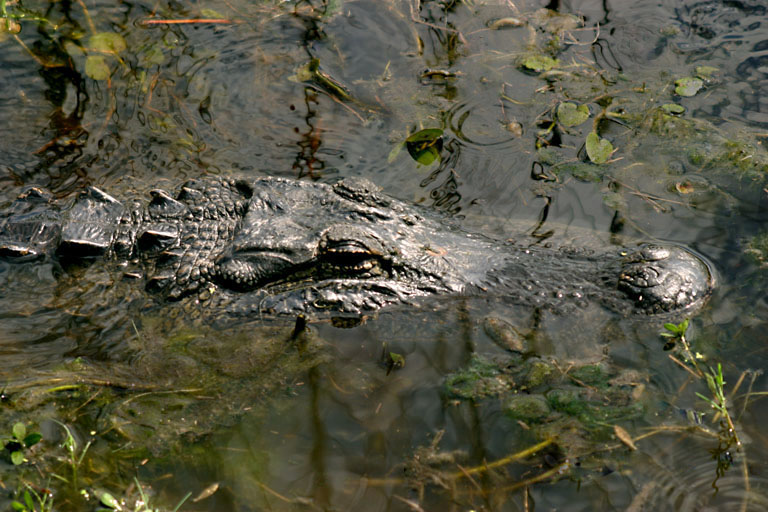
\includegraphics[height=\paperheight]{figure/GatorHeadModified.jpg}}
\begin{frame}[plain,c]
% \vspace*{-0.1in}
\begin{center}
  {\color[RGB]{241,243,186}
{\huge EEL6935 Course Project Proposal\\
    \vspace*{0.5em}
    Sentiment Analysis}\\
  \vspace*{1.8in}
    Caleb Bryent \& Jixin Feng \\
    \vspace*{1em}
  \begin{tabular}{cc}
  University of Florida
   \end{tabular}
}
  \end{center}
\hoffset=0em
\end{frame}}

\begin{frame}
\frametitle{Background}
    \begin{columns}
    \begin{column}{0.5\textwidth}
    \begin{itemize}
        \item Tremendous volume of unstructured text generated everyday
        \item 40ZB ($40\times 10^{21}$bytes) by year 2020, 50-fold from 2010\footnotemark
        \item generated from news media, social networks, medical records, 
            business transactions\ldots
        \item effective processing method is needed
    \end{itemize}
    \end{column}
    \begin{column}{0.5\textwidth}
    \center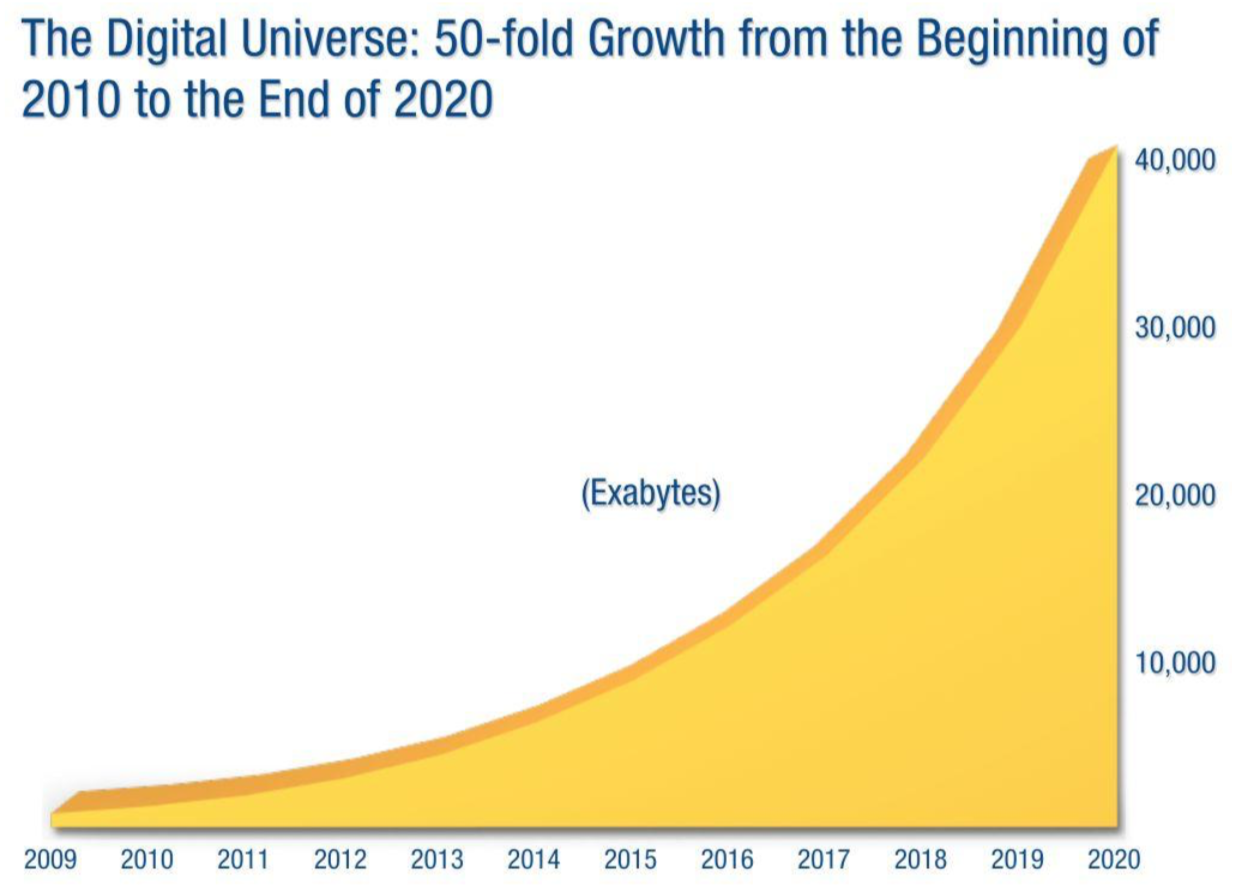
\includegraphics[width=\textwidth]{figure/data_growth_2020}
    \end{column}
    \end{columns}
    \footnotetext[1]{Gantz, J., \& Reinsel, D. (2012). The digital universe in 2020: Big data, bigger digital shadows, and biggest growth in the far east. IDC iView: IDC Analyze the future, 2007(2012), 1-16.}
\end{frame}

\begin{frame}
\frametitle{Sentiment Analysis}
    Goal: assign pre-defined labels to a sentence, categorize opinion.
    $$f:\mathcal{D}\rightarrow\mathcal{L}$$
    \begin{itemize}
        \item $\mathcal{D}=\{d_0, d_1,\ldots, d_{n-1}\}$ is the set of sentence
        \item $\mathcal{L}=\{l_0, l_1,\ldots, l_{k-1}\}$ is the set of labels.
    \end{itemize}
    In the domain of sentiment analysis, $\mathcal{L}$ can be binary:
    \begin{itemize}
    \item Like/Dislike
    \item Agree/Disagree
    \item etc.
    \end{itemize}
\end{frame}

\begin{frame}
\frametitle{Evaluation}
\begin{columns}
    \begin{column}{0.65\textwidth}
    The performance can be measured by $F_1$ Score:
    $$F_1=\frac{2}{\frac{1}{r}+\frac{1}{p}}=\frac{2pr}{p+r}$$
    \begin{itemize}
        \item Precision: $p=\frac{tpr}{tpr+fpr}$
        \item Recall: $r=\frac{tpr}{tpr+fnr}$
    \end{itemize}
    \end{column}
    \begin{column}{0.35\textwidth}
        \center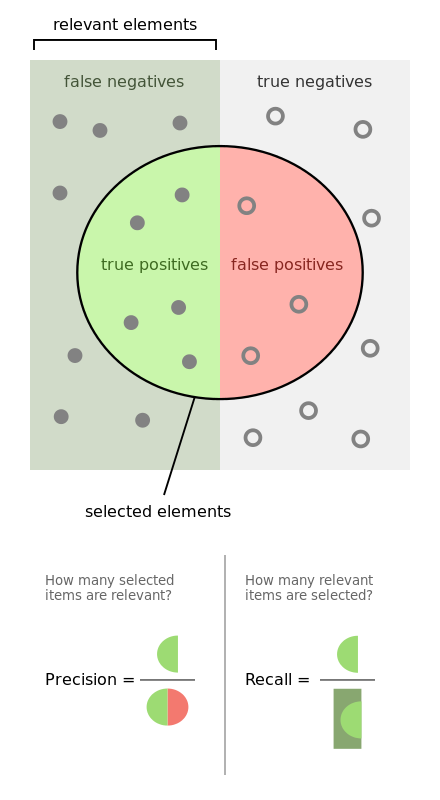
\includegraphics[width=\textwidth]{figure/precision_recall}
    \end{column}
    \end{columns}
    \footnotetext{figure credit: \url{https://en.wikipedia.org/wiki/F1_score}}
\end{frame}

\begin{frame}
\frametitle{Compare performance}
    \begin{columns}
    \begin{column}{0.5\textwidth}
    \center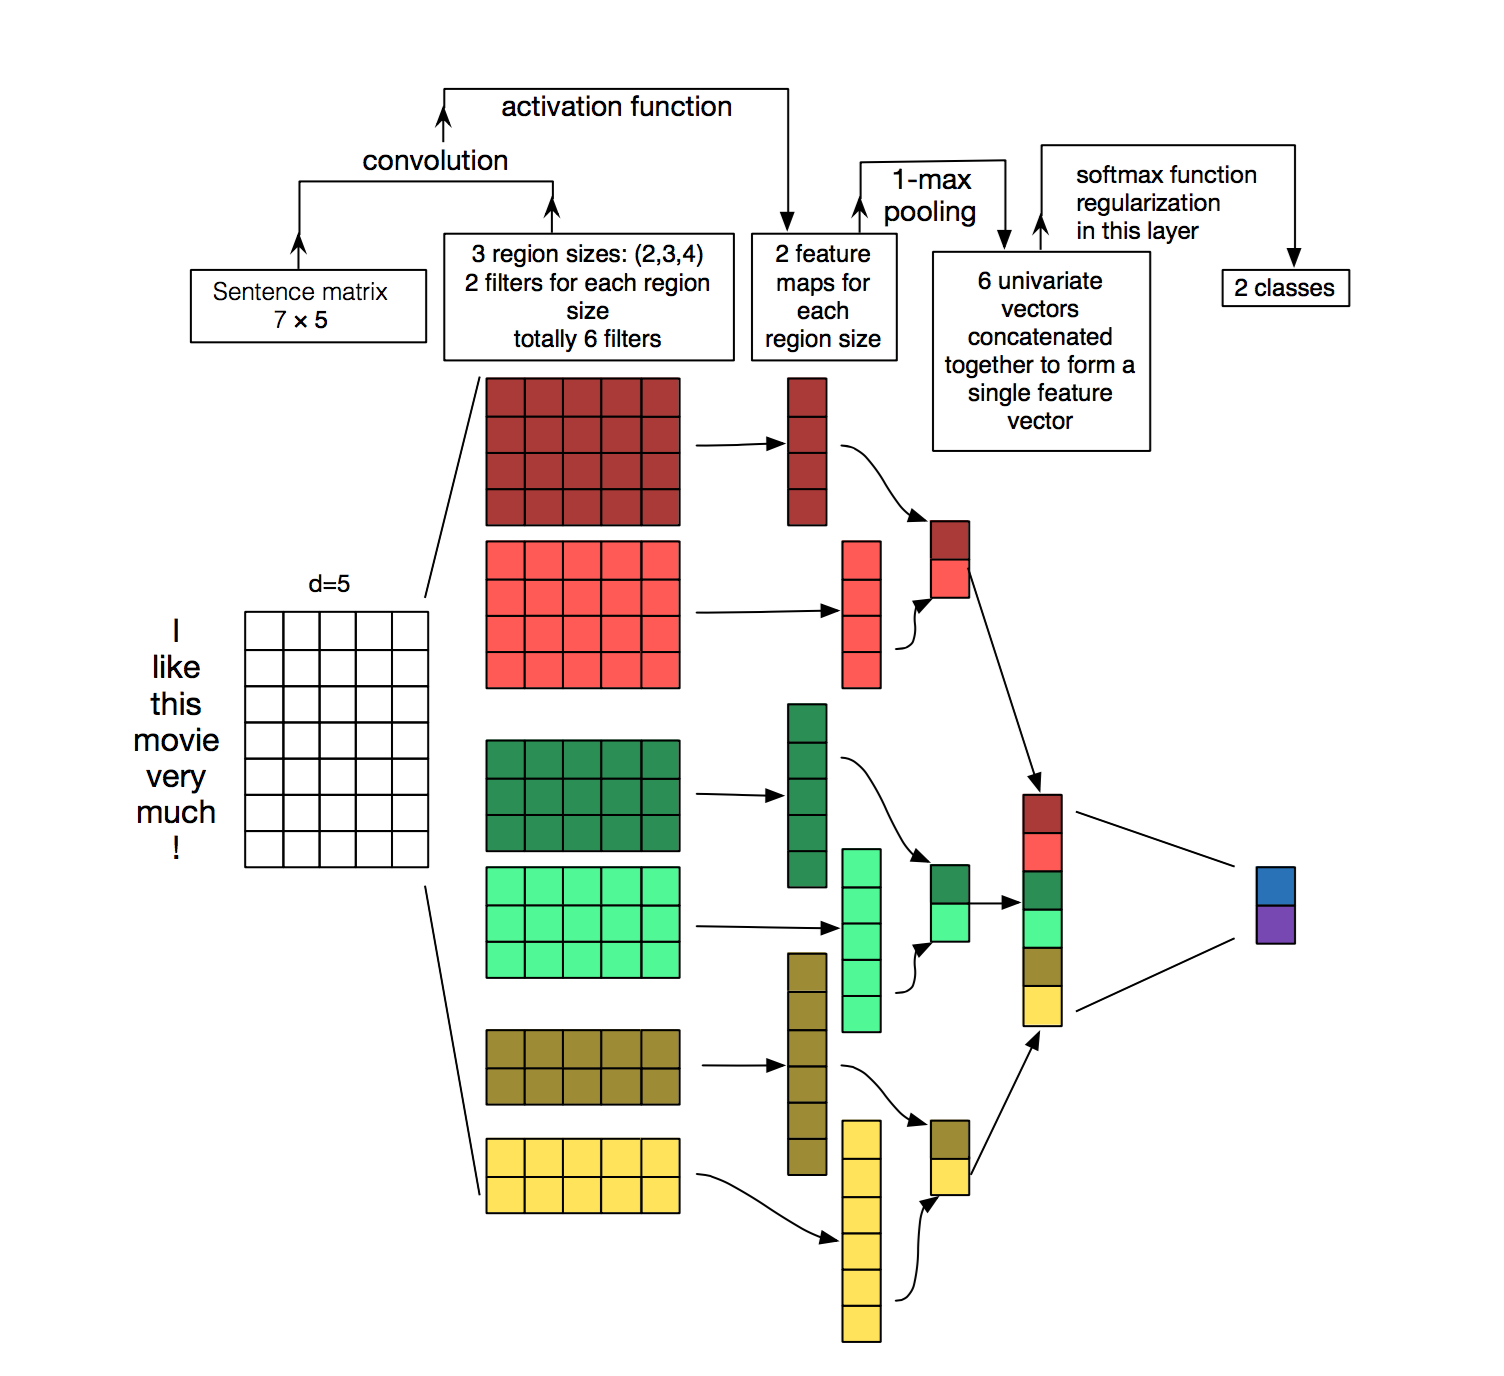
\includegraphics[width=\textwidth]{figure/sc_cnn}
    \end{column}
    \begin{column}{0.5\textwidth}
    \begin{itemize}
        \item Historically via naive Bayes, nearest neighbor, decision trees, SVM, etc.
        \item Build baseline model with Logistic Regression
        \item Implement CNN model and compare performance
        \item If time allows, compare with LSTM model too
    \end{itemize}
    \end{column}
    \end{columns}
    \footnotetext{figure credit: http://www.wildml.com/2015/11/understanding-convolutional-neural-networks-for-nlp/}
\end{frame}

\begin{frame}
\frametitle{Baseline Model: Logistic Regression}
    Represent text using Vector Space Model/Bag-of-Words Model
    \begin{itemize}
        \item Define word set $$\mathcal{W}=\{w_0, w_1,\ldots, w_{m-1}\}$$
        \item Let $n_j(d_i)$ be a metric of word $w_j$ in sentence $d_i$
        \item Each sentence can be vectorized
        $$\bar{d_i}=(n_0(d_i),n_1(d_i),\ldots,n_{m-1}(d_i))$$
        \item $n_j(d_i)$ can be either occurrence or frequency
    \end{itemize}
\end{frame}

\begin{frame}
\frametitle{Baseline Model: Logistic Regression}
    \begin{itemize}
    \item $\hat{y} = \sigma(S(x^T_i W +b))$
    \item $S(x) = \frac{1}{1+e^{-x}}$
    \item $W$ is a $N \times C$ weight matrix, 
    $N$ is number of words, $C$ is number of class
    \item $\sigma (x)_{j}={\frac {e^{x_{j}}}{\sum _{i=1}^{N}e^{x_{i}}}}$
    \item $b$ is a $C \times 1$ bias
    \item pick $i=argmax(\hat{y}_i)$
    \end{itemize}
    train the model using
    Stochastic Gradient Descent
\end{frame}

\begin{frame}
\frametitle{CNN Model: Sentence}
    We model a sentence as:
    $$x_{1:n} = x_1 \oplus x_2 \oplus ... \oplus x_n$$
    \begin{itemize}
        \item $x_{i} \in \mathbb{R}^k$: dimensional word vector representing the $i$-th word in the sentence
        \item $\oplus$ signifies concatenation
        \item $x_{i:i+j}$: concatenating word vectors $x_i, x_{i+1}, ... , x_{i+j}$
    \end{itemize}
\end{frame}

\begin{frame}
\frametitle{CNN Model: Convolution}
    Convolution operator is defined as:
    $$c_i = f(W \cdot x_{i:i_{h-1}} + b)$$
    \begin{itemize}
        \item $W \in \mathbb{R}^{hk}$: filter
        \item $h$: window size
        \item $b$: bias term
        \item $f$: signifies a non linear function
    \end{itemize}
    Feature map
    $$c = [c_1, c_2, ... ,x_{n-h+1}], c \in \mathbb{R}^{n-h+1}$$
    is then applied to 
    $$x_{1:h}, x_{2:h+1}, ... ,x_{n-h+1:n}$$
\end{frame}

\begin{frame}
\frametitle{CNN Model: Output}
    Dropout on the penultimate layer 
    $$z = [\hat{c}_1,...,\hat{c}_m], \hat{c}=\operatorname{max}\{c\}$$
    The final output is:
    $$y = W \cdot (z \circ r) + b$$
    \begin{itemize}
    \item $\circ$: element-wise multiplication operator
    \item $r \in \mathbb{R}^m$: masking vector of Bernoulli random variables
    \end{itemize}
\end{frame}

\begin{frame}
\frametitle{LSTM Model}
    $$
    \begin{bmatrix} 
    i_t\\f_t\\o_t\\c_t 
    \end{bmatrix} = 
    \begin{bmatrix}
    \sigma\\\sigma\\\sigma\\\tanh
    \end{bmatrix}
    S[h_{t-1},x_t]
    $$
\end{frame}

\begin{frame}
\frametitle{Simulation Platform Specs}
    \begin{itemize}
        \item Propose using the Stanford Large Movie Review Dataset
        \begin{itemize}
            \item 50,000 highly polar movie reviews
        \end{itemize}
        \item Score each movie review as either positive or negative
        \item Use a 60/20/20 split for training, development, and testing
        \item Code in Python with Tensorflow
        \item simulations will be conducted on computers with 
        \begin{itemize}
            \item 3.1GHz Intel Core i7 CPU with 8MB cache
            \item nVidia GTX 1050 GPU with 4GB Memory
            \item 16GB RAM
            \item Ubuntu 14.04 LTS
        \end{itemize}
    \end{itemize}
\end{frame}

\begin{frame}
\frametitle{Project Progress}
    \begin{description}
        \item[\CheckedBox] Choose topic
        \item[\CheckedBox] Write proposal
        \item[\CheckedBox] Gather dataset
        \item[\CheckedBox] Build baseline model with Logistic Regression
        \item[\CheckedBox] Write mid-term report 
        \item[$\Box$] Build CNN model
        \item[$\Box$] (stretch) Build LSTM model
        \item[$\Box$] (stretch) Build web interface
        \item[$\Box$] Write project documentation
        \item[$\Box$] Write final report
    \end{description}
\end{frame}

\begin{frame}
\frametitle{Weekly Plan}
\begin{center}
    \begin{tabular}{| l | p{7cm} |}
        \hline
        Week & Plan \\ \hline
        1-3 & Read paper and select project topic \\ \hline
        4 & Write project proposal and make slides \\ \hline
        6-8 & Build project baseline model and finalize design \\ \hline
        9 & Write midterm project report and make slides \\ \hline
        10-13 & Build CNN model and work on stretched goals \\ \hline
        14-15 & Finalize course project, collect data and write final report \\ \hline
        \end{tabular}
    \end{center}
\end{frame}

\begin{frame}
\center{\huge Thank You!}
\center Questions?
\end{frame}
\end{document}
